% Fig 3 (fig:mechanism): standalone source for the paper figure.
% Build: pdflatex mechanism.tex  ->  mechanism.pdf  (see build_figures.sh)
\documentclass[border=2pt]{standalone}
\usepackage[T1]{fontenc}
\usepackage{amsmath,amssymb}
\usepackage{tikz}
\usetikzlibrary{shapes.geometric, arrows.meta, positioning, patterns, calc}
% Okabe-Ito colorblind-safe palette (Wong 2011, Nature Methods)
\definecolor{oiblue}{HTML}{0072B2}
\definecolor{oiorange}{HTML}{E69F00}
\definecolor{oiskyblue}{HTML}{56B4E9}
\definecolor{oigray}{HTML}{999999}
\definecolor{oivermillion}{HTML}{D55E00}
\definecolor{oigreen}{HTML}{009E73}
\definecolor{oipurple}{HTML}{CC79A7}
\begin{document}
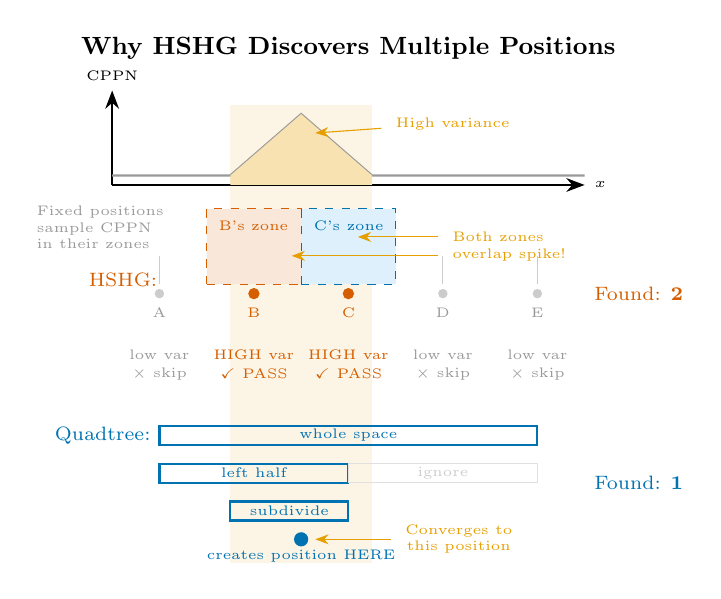
\begin{tikzpicture}[scale=0.6]
    % Title
    \node[font=\small\bfseries] at (6, 10.2) {Why HSHG Discovers Multiple Positions};
    % Vertical band showing spike width
    \fill[oiorange!10] (3.5, -0.7) rectangle (6.5, 9);
    % === TOP: CPPN with axes ===
    \draw[-{Stealth}, thick] (1, 7.3) -- (11, 7.3) node[right, font=\tiny] {$x$};
    \draw[-{Stealth}, thick] (1, 7.3) -- (1, 9.3) node[above, font=\tiny] {CPPN};
    \draw[thick, oigray] (1, 7.5) -- (3.5, 7.5) -- (5, 8.8) -- (6.5, 7.5) -- (11, 7.5);
    \fill[oiorange!30] (3.5, 7.3) -- (3.5, 7.5) -- (5, 8.8) -- (6.5, 7.5) -- (6.5, 7.3) -- cycle;
    \node[font=\tiny, oiorange, anchor=west] at (6.8, 8.6) {High variance};
    \draw[-{Stealth}, oiorange, thin] (6.7, 8.5) -- (5.3, 8.4);
    % === MIDDLE: HSHG fixed grid positions with neighborhoods ===
    \node[font=\scriptsize, oivermillion, anchor=west] at (0.3, 5.3) {HSHG:};
    \foreach \x in {2, 4, 6, 8, 10} {
        \draw[oigray!50] (\x, 5.8) -- (\x, 5.2);
    }
    \fill[oigray!50] (2, 5) circle (0.1);
    \fill[oivermillion] (4, 5) circle (0.12);
    \fill[oivermillion] (6, 5) circle (0.12);
    \fill[oigray!50] (8, 5) circle (0.1);
    \fill[oigray!50] (10, 5) circle (0.1);
    \node[font=\tiny, oigray] at (2, 4.6) {A};
    \node[font=\tiny, oivermillion] at (4, 4.6) {B};
    \node[font=\tiny, oivermillion] at (6, 4.6) {C};
    \node[font=\tiny, oigray] at (8, 4.6) {D};
    \node[font=\tiny, oigray] at (10, 4.6) {E};
    \fill[oivermillion!15] (3, 5.2) rectangle (5, 6.8);
    \draw[oivermillion, dashed] (3, 5.2) rectangle (5, 6.8);
    \node[font=\tiny, oivermillion, anchor=north west] at (3.05, 6.75) {B's zone};
    \fill[oiskyblue!20] (5, 5.2) rectangle (7, 6.8);
    \draw[oiblue, dashed] (5, 5.2) rectangle (7, 6.8);
    \node[font=\tiny, oiblue, anchor=north east] at (6.95, 6.75) {C's zone};
    \node[font=\tiny, oigray, align=left, anchor=west] at (-0.8, 6.4) {Fixed positions \\ sample CPPN \\ in their zones};
    \node[font=\tiny, oiorange, align=left, anchor=west] at (8, 6.0) {Both zones\\overlap spike!};
    \draw[-{Stealth}, oiorange, thin] (7.9, 6.2) -- (6.2, 6.2);
    \draw[-{Stealth}, oiorange, thin] (7.9, 5.8) -- (4.8, 5.8);
    \node[font=\tiny, oigray] at (2, 3.7) {low var};
    \node[font=\tiny, oigray] at (2, 3.3) {$\times$ skip};
    \node[font=\tiny, oivermillion] at (4, 3.7) {HIGH var};
    \node[font=\tiny, oivermillion] at (4, 3.3) {$\checkmark$ PASS};
    \node[font=\tiny, oivermillion] at (6, 3.7) {HIGH var};
    \node[font=\tiny, oivermillion] at (6, 3.3) {$\checkmark$ PASS};
    \node[font=\tiny, oigray] at (8, 3.7) {low var};
    \node[font=\tiny, oigray] at (8, 3.3) {$\times$ skip};
    \node[font=\tiny, oigray] at (10, 3.7) {low var};
    \node[font=\tiny, oigray] at (10, 3.3) {$\times$ skip};
    \node[font=\scriptsize, oivermillion, right] at (11, 5) {Found: \textbf{2}};
    % === BOTTOM: Quadtree comparison ===
    \node[font=\scriptsize, oiblue] at (0.8, 2) {Quadtree:};
    \draw[oiblue, thick] (2, 1.8) rectangle (10, 2.2);
    \node[font=\tiny, oiblue] at (6, 2) {whole space};
    \draw[oiblue, thick] (2, 1) rectangle (6, 1.4);
    \draw[oigray!30] (6, 1) rectangle (10, 1.4);
    \node[font=\tiny, oiblue] at (4, 1.2) {left half};
    \node[font=\tiny, oigray!50] at (8, 1.2) {ignore};
    \draw[oiblue, thick] (3.5, 0.2) rectangle (6, 0.6);
    \node[font=\tiny, oiblue] at (4.75, 0.4) {subdivide};
    \fill[oiblue] (5, -0.2) circle (0.15);
    \node[font=\tiny, oiblue] at (5, -0.55) {creates position HERE};
    \node[font=\tiny, oiorange, align=center, anchor=west] at (7, -0.2) {Converges to\\this position};
    \draw[-{Stealth}, oiorange, thin] (6.9, -0.2) -- (5.3, -0.2);
    \node[font=\scriptsize, oiblue, right] at (11, 1) {Found: \textbf{1}};
\end{tikzpicture}
\end{document}
